\documentclass{ximera}

\begin{document}
	\author{Stitz-Zeager}
	\xmtitle{The Shape of Graphs}


\mfpicnumber{1}

\opengraphsfile{AppDerivatives}

\setcounter{footnote}{0}

\label{AppDerivatives}

We know if $f$ is differentiable at $x=a$ then the graph of  $f$ is \textbf{locally linear} at $x=a$ and $f'(a)$ is the \textbf{slope} of the tangent line at the point $(a, f(a))$.  In this section, we explore how local behavior near a point can be extrapolated to global behavior over an interval.  First, we review Definition \ref{incdeccnstdefn} from Section \ref{ConstantandLinearFunctions}:

\medskip

%% \colorbox{ResultColor}{\bbm

\begin{defnrecall}

Let $f$ be a function defined on an interval $I$.  Then $f$ is said to be:

\begin{itemize}

\item  \textbf{increasing} on $I$ if, whenever $a < b$, then $f(a) < f(b)$.   (i.e., as inputs increase, outputs \textbf{increase}.)

\textbf{NOTE:}  The graph of an increasing function  \textbf{rises} as one moves from left to right.

\item  \textbf{decreasing} on $I$ if, whenever $a < b$, then $f(a) > f(b)$.  (i.e., as inputs increase, outputs \textbf{decrease}.)

\textbf{NOTE:}  The graph of a decreasing function \textbf{falls} as one moves from left to right.

\item  \textbf{constant} on $I$ if $f(a) = f(b)$ for all $a$, $b$ in $I$.  (i.e., outputs don't change with inputs.)

\textbf{NOTE:}  The graph of a function that is constant over an interval is a horizontal line.

\end{itemize}

\end{defnrecall}

%% \ebm}


\medskip

Suppose a function satisfies $f'(x)  > 0$ for all $x$ in an open interval\footnote{We've defined derivatives  as two-sided limits, so an open interval here guarantees enough `room' on either side of any given number to take such a limit.} $I$.   Then we know that not only is the graph of $f$ locally linear on $I$, but the slopes of all of the tangent lines are positive.  This means that all of the tangent lines are increasing so it stands to reason that the function $f$ is likewise increasing on $I$. In other words, if a function is \textbf{locally} increasing on $I$,  then it is \textbf{globally} increasing on $I$ as well.

\medskip

We can apply the same reasoning above to situations where $f'(x)<0$ for all $x$ in $I$, which implies $f$ is decreasing on $I$ or $f'(x) = 0$ on $I$, which implies $f$ is constant on $I$.  In Calculus, you'll learn this fact is a consequence of the Mean Value Theorem.\footnote{which Carl thinks is the actual `Fundamental Theorem of Calculus' since it relates local and global behavior \ldots}  In this text, we'll just accept the following theorem is true and hope we've done enough hand-waving to deem it reasonable.

\medskip

%% \colorbox{ResultColor}{\bbm

\begin{theorem}  \label{firstderivatveandgraphs}   Suppose $f$ is differentiable on an open interval $I$:

\begin{itemize}

\item If $f'(x) > 0$ for all $x$ in $I$, then $f$ is increasing on $I$.  

\item If $f'(x) < 0$ for all $x$ in $I$, then $f$ is decreasing on $I$. 

\item If $f'(x) = 0$ for all $x$ in $I$, then $f$ is constant on $I$.


\end{itemize}

\end{theorem}
%% \ebm}

\pagebreak


Theorem \ref{firstderivatveandgraphs} may be visualized as follows:

\begin{itemize}

\item  $f'(x) > 0$  for all $x$ in $I$:

\begin{center}

\begin{multicols}{2}

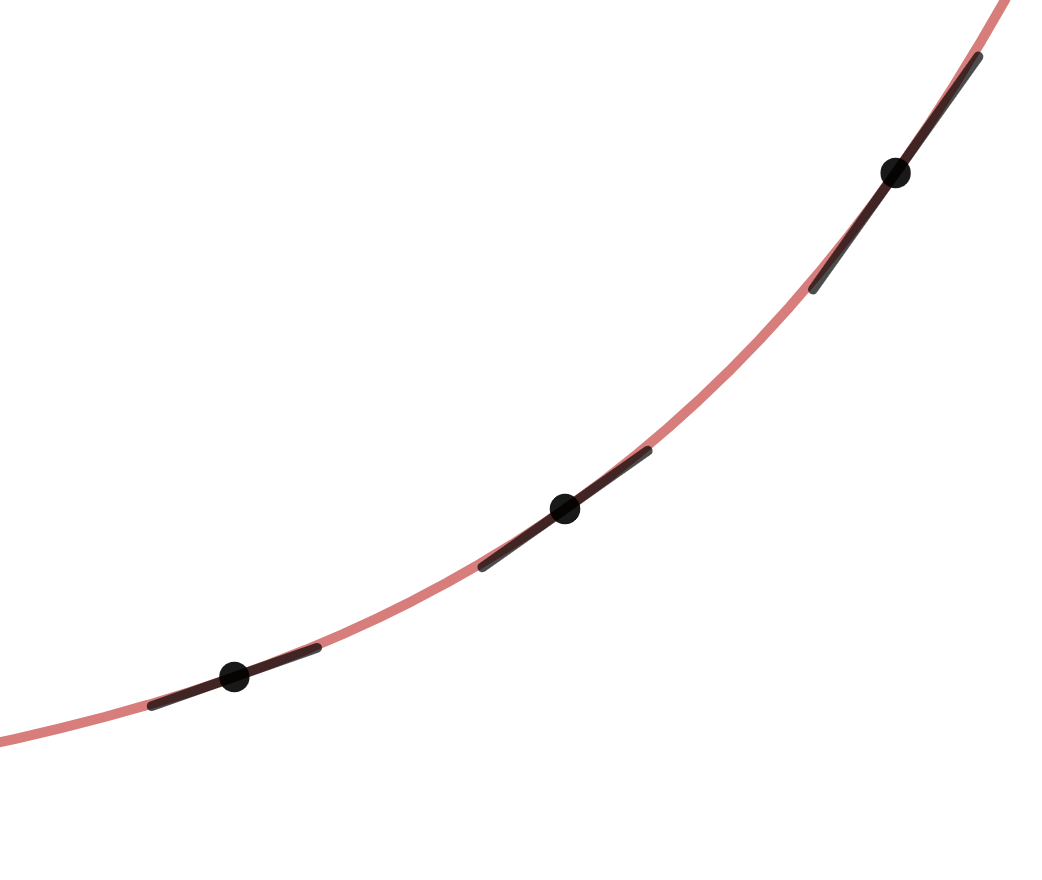
\includegraphics[width=1.5in]{./AppDerivativesGraphics/IncCU.png} 

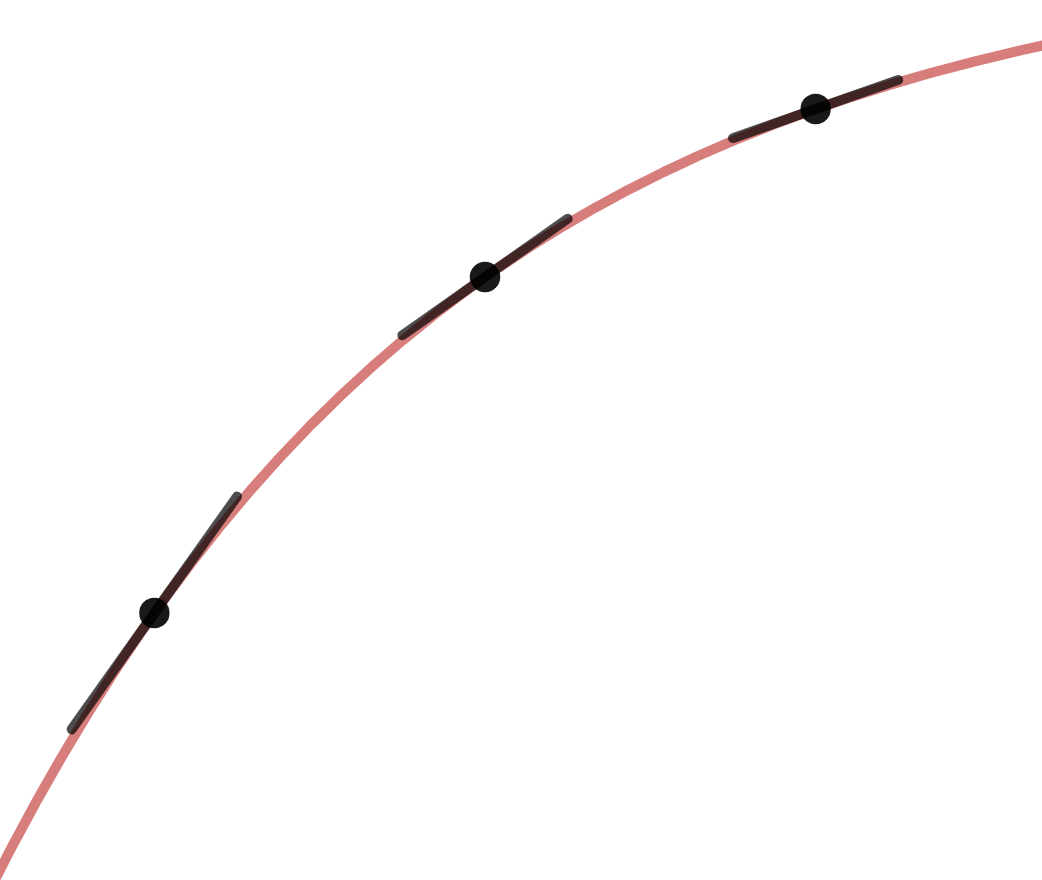
\includegraphics[width=1.5in]{./AppDerivativesGraphics/IncCD.png} 

\end{multicols}

\end{center}

\item  $f'(x) < 0$  for all $x$ in $I$:


\begin{center}

\begin{multicols}{2}

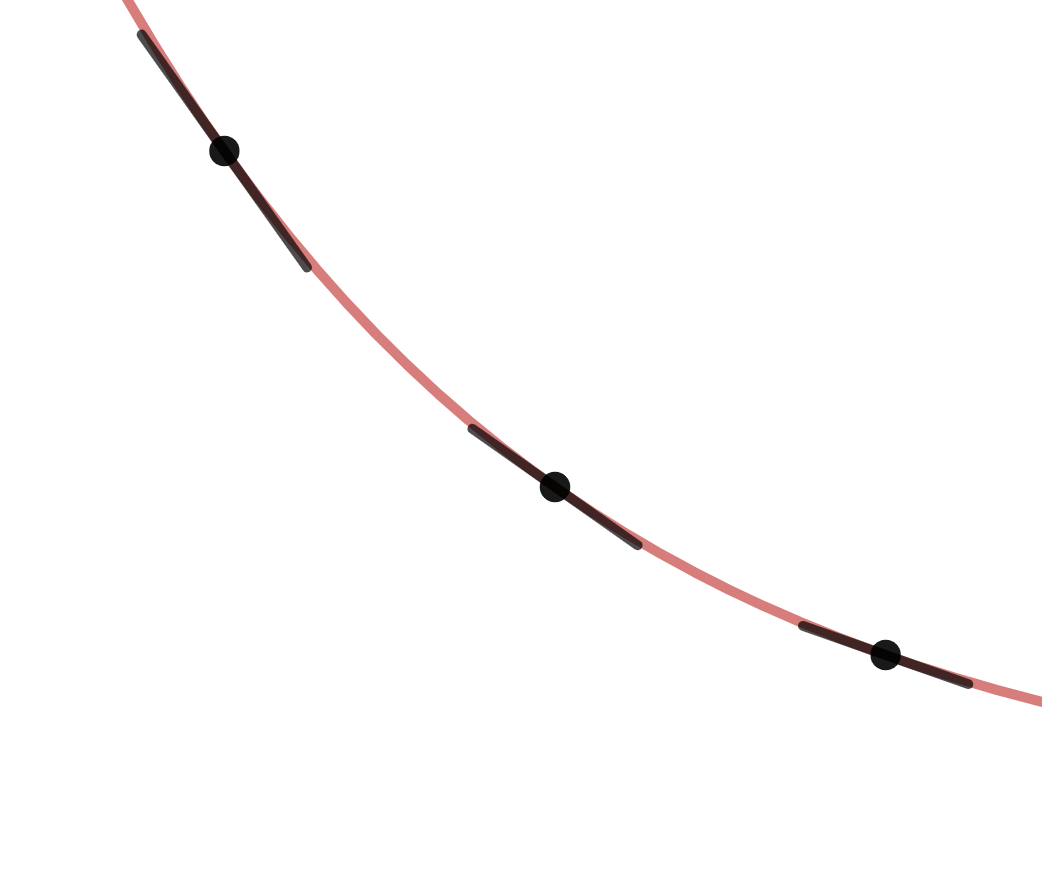
\includegraphics[width=1.5in]{./AppDerivativesGraphics/DecCU.png} 

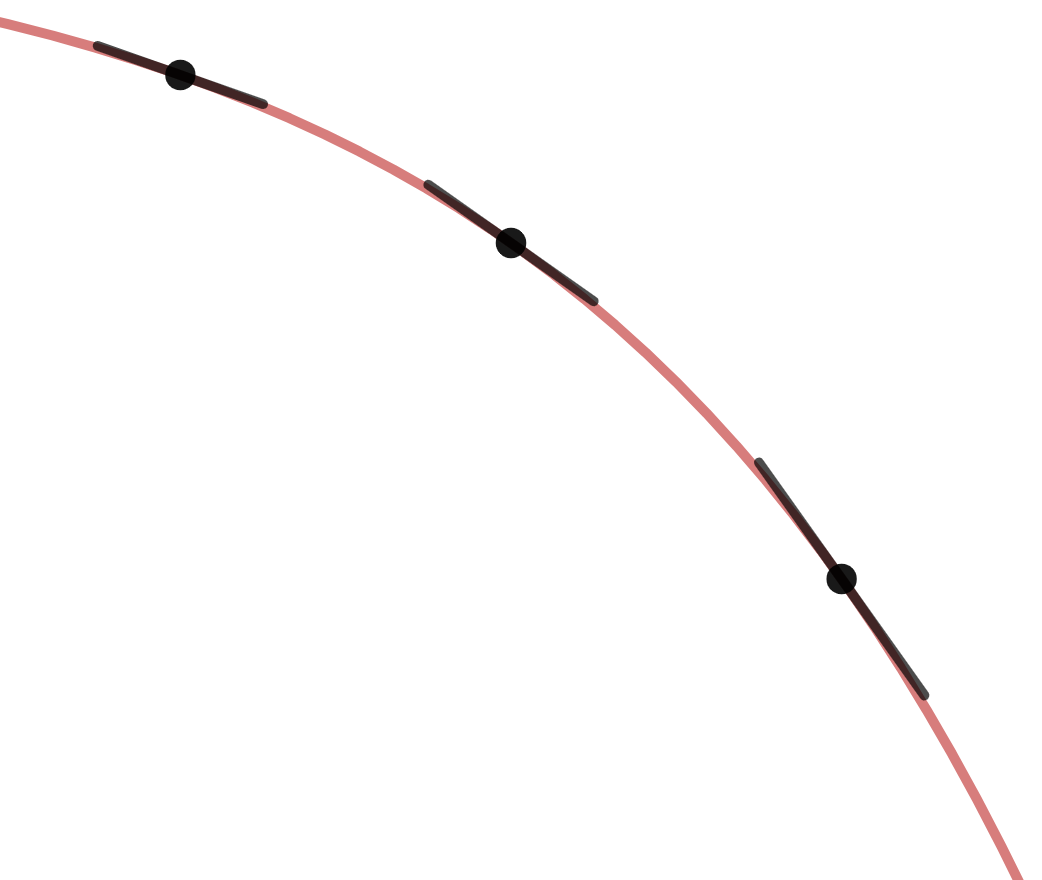
\includegraphics[width=1.5in]{./AppDerivativesGraphics/DecCD.png} 

\end{multicols}

\end{center}


\item $f'(x) = 0$  for all $x$ in $I$:

\begin{center}

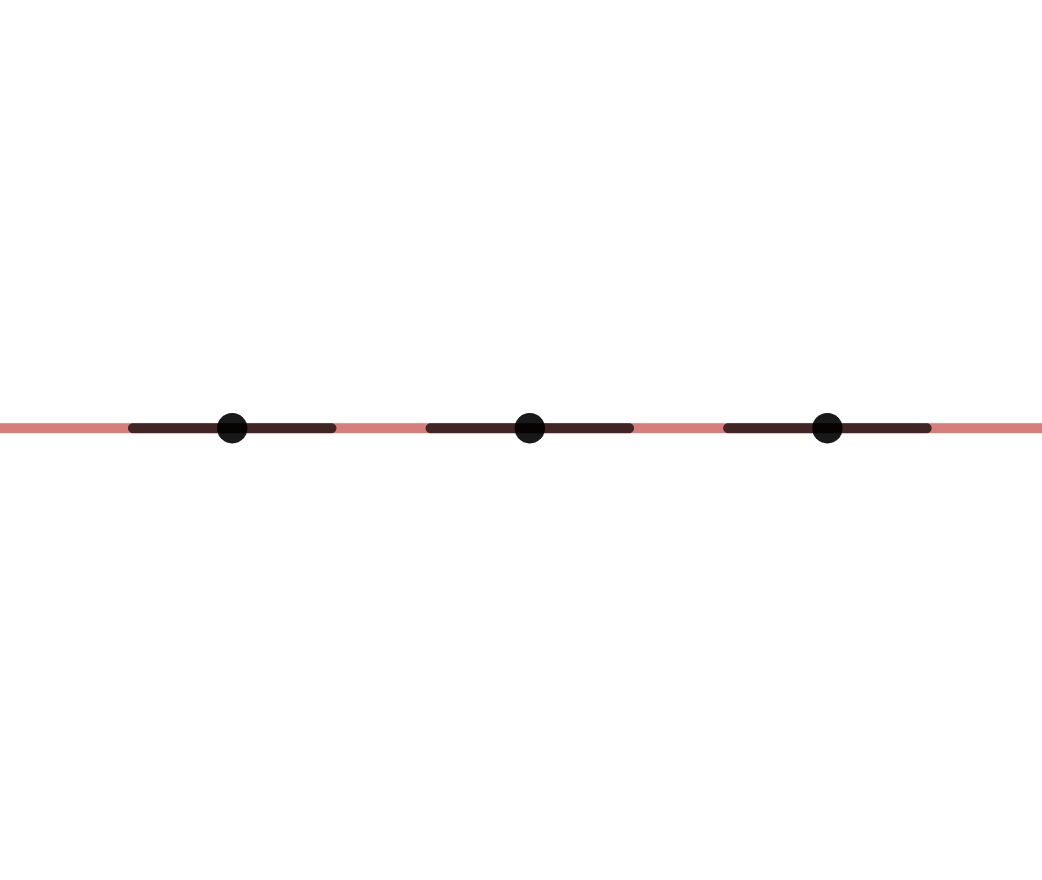
\includegraphics[width=1.5in]{./AppDerivativesGraphics/Constant.png} 

\end{center}

\end{itemize}

We can use Theorem \ref{firstderivatveandgraphs} to help us determine the (open) intervals over which a function $f$ is increasing, decreasing, and constant by making a sign diagram for the derivative $f'$. 

\medskip

In order to avoid us having to go through the (somewhat lengthy) process of finding $f'(x)$ using Definition \ref{derivativefcndefn}, we'll just use some properties of derivatives from Calculus behind the scenes and present you with both a function and its derivative.  It's time for an example.

\medskip

\begin{example}\label{polyincdec}  Let  $f(x) = x^3 - 3x^2 - 9x+5$.  Use the fact that $f'(x) = 3x^2-6x-9$  to find the open intervals over which $f$ is increasing, decreasing, and constant.  Check your answer graphically.

\medskip


{\bf Solution.}   To make use of  Theorem \ref{firstderivatveandgraphs}, we make a sign diagram for $f'(x)$.  Since $f'$ is a polynomial, $f'$ is continuous so the per the Intermediate Value Theorem, Theorem \ref{IVT}, $f'$ will only change sign on either side of zeros.  Hence, our first step is to solve  $f'(x) = 0$.  


\medskip

We are given  $f'(x) = 3x^2-6x-9$.   Solving $f'(x) =  3x^2-6x-9 = 0$  gives  $3(x^2-2x-3) = 0$ or   $3(x-3)(x+1) = 0$.  We get two solutions:  $x = -1$ and $x = 3$ which divides the $x$-axis into three regions:  $x< -1$, $-1<x<3$ and $x>3$. 

\medskip

Next we select a test value in each of these three regions to determine the sign of $f'(x)$.  For the interval $x<-1$, we select $x = -3$:   $f'(-3) = 3(-3)^2-6(-3)-9 = (+)$.  For $-1<x<3$, we select $x = 0$:  $f'(0) =  3(0)^2-6(0)-9 = (-)$. Finally, for $x>3$, we select $x = 4$:  $f'(4) = 3(4)^2-6(4)-9  = (+)$.

\medskip

Below on the left is a sign diagram for $f'(x)$ and on the right is what this means for the graph of $y=f(x)$:

\begin{center}

\begin{multicols}{2}

\begin{mfpic}[15]{-6}{6}{-2}{2}
\arrow \reverse \arrow \polyline{(-5,0),(5,0)}
\xmarks{-2,2}
\arrow \polyline{(-3.5,-1.5),(-3.5,-0.5)}
\arrow \polyline{(0,-1.5),(0,-0.5)}
\arrow \polyline{(3.5,-1.5),(3.5,-0.5)}
\tlpointsep{4pt}
\axislabels {x}{{$-1 \hspace{7pt}$} -2, {$3$} 2}
\tlabel[cc](-3.5,1){$(+)$}
\tlabel[cc](-2,1){$0$}
\tlabel[cc](0,1){$(-)$}
\tlabel[cc](2,1){$0$}
\tlabel[cc](3.5,1){$(+)$}
\tlabel[cc](-3.75,-2.25){$-3$}
\tlabel[cc](0,-2.25){$0$}
\tlabel[cc](3.6,-2.25){$4$}
\tlabel[cc](6,1){$f'(x)$}
\tlabel[cc](6,-1){$x$}
%\tlabel[cc](6,0){$\infty$}
%\tlabel[cc](-6,0){$-\infty$}
\end{mfpic}

\begin{mfpic}[15]{-6}{6}{-2}{2}
\arrow \reverse \arrow \polyline{(-5,0),(5,0)}
\xmarks{-2,2}
%\arrow \polyline{(-3.5,-1.5),(-3.5,-0.5)}
%\arrow \polyline{(0,-1.5),(0,-0.5)}
%\arrow \polyline{(3.5,-1.5),(3.5,-0.5)}
\tlpointsep{4pt}
\axislabels {x}{{$-1\hspace{7pt}$} -2, {$3$} 2}
\tlabel[cc](-3.5,1){$\nearrow$}
\tlabel[cc](-2,1){$\rightarrow$}
\tlabel[cc](0,1){$\searrow$}
\tlabel[cc](2,1){$\rightarrow$}
\tlabel[cc](3.5,1){$\nearrow$}
%\tlabel[cc](-3.75,-2.25){$-3$}
%\tlabel[cc](0,-2.25){$0$}
%\tlabel[cc](3.6,-2.25){$4$}
\tlabel[cc](6,1){$f(x)$}
\tlabel[cc](6,-1){$x$}
%\tlabel[cc](6,0){$\infty$}
%\tlabel[cc](-6,0){$-\infty$}
\end{mfpic}


\end{multicols}
\end{center}

We find $f$ is increasing on $(-\infty, -1)$ and again on $(3, \infty)$ while  $f$ is decreasing on $(-1,3)$.  At the points $x = -1$ and $x=3$, we have $f'(x) = 0$ so the graph of $f$ is locally flat there.  

\medskip

Since $f$ changes from increasing just to the left of $x=-1$ to decreasing just to the right of $x=-1$, it stands to reason that $f$ has a local maximum at $x=-1$.  This is indeed the case and we find that the local maximum value is  $f(-1) = (-1)^3 - 3(-1)^2 - 9(-1)+5 = 10$.

\medskip

Similarly, since $f$ changes from decreasing just to the left of $x=3$ to increasing just to the right of $x=3$, $f$ has a local minimum at $x=3$.  The local minimum value is $f(3) = (3)^3 - 3(3)^2 - 9(3)+5 = -22$.

\medskip


A quick check using desmos confirms our results.

\medskip

\centerline{ 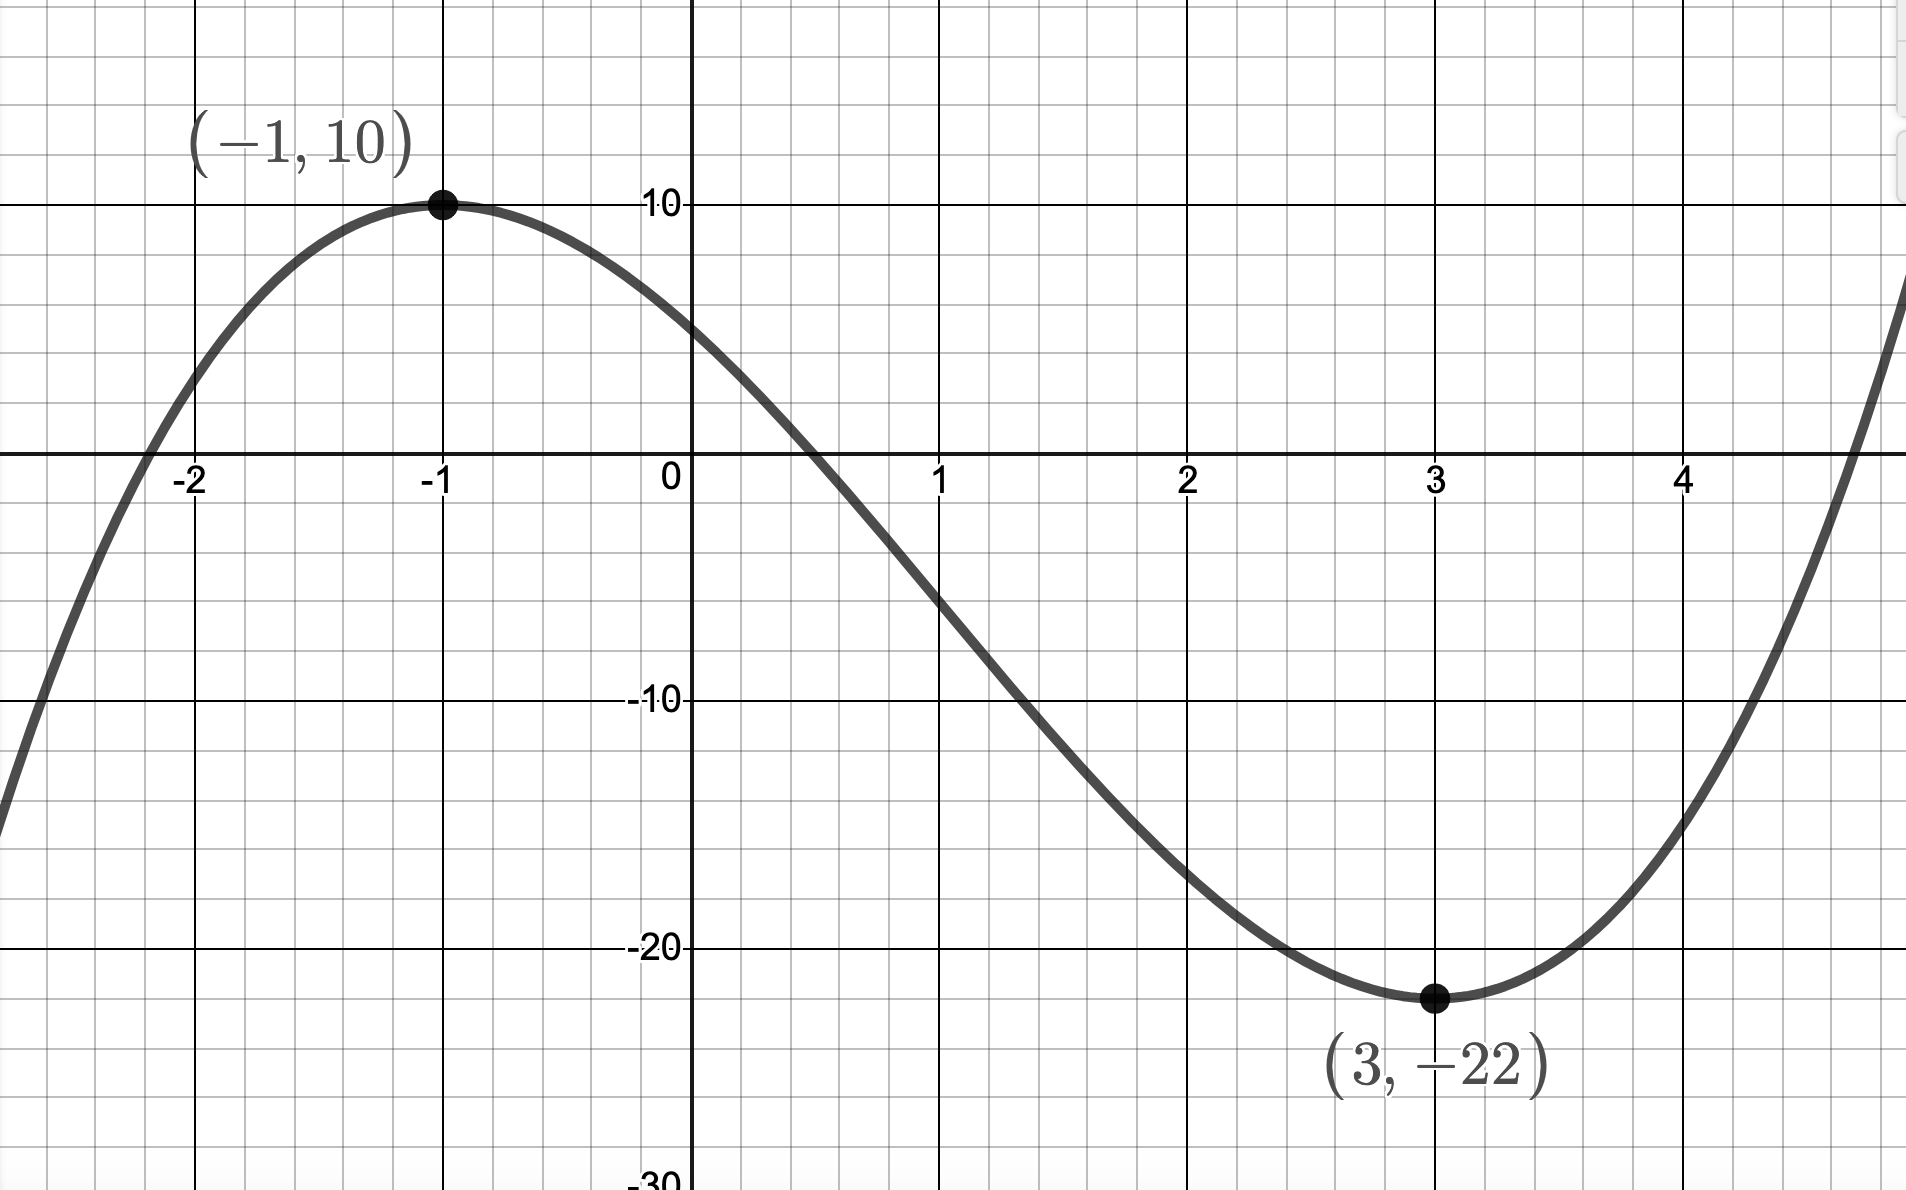
\includegraphics[width=4in]{./AppDerivativesGraphics/IncDecPoly.png}}

\hfill \qed

\end{example}

We generalize our observations about local extrema in the following result.

\medskip

%% \colorbox{ResultColor}{\bbm

\begin{theorem}  \label{firstderivatvetest}   \textbf{The (First)\footnote{Why `First'?  Stay tuned \ldots} Derivative Test for Local Extema:}  Let $f$ be continuous on an open interval $I$ containing a critical number $c$.\footnote{Recall this means $f'(c) = 0$ or $f'(c)$ does not exist.}  If $f$ is differentiable on $I$, except possibly at $c$, then  

\medskip

\begin{itemize}

\item If $f'(x)$ changes from $(+)$ for $x<c$ to $(-)$ for $x>c$, $f$ has a local maximum at $x=c$.

\item If $f'(x)$ changes from $(-)$ for $x<c$ to $(+)$ for $x>c$, $f$ has a local minimum at $x=c$.

\item If $f'(x)$ doesn't change sign going from $x<c$ to $x>c$, $f$ does not have a local extremum at $x=c$.

\end{itemize}

\end{theorem}
%% \ebm}

\medskip

\begin{example} \label{powerfcnincdec} Let $f(x) = x^{4/3} - 4x^{1/3}$. Use the fact that $f'(x) = \frac{4}{3} x^{1/3} - \frac{4}{3} x^{-2/3}$ to help you find:

\begin{enumerate}

\item the open intervals over which $f$ is increasing, decreasing, and constant.

\item the local extrema.

\end{enumerate}

{\bf Solution.}    \begin{enumerate}  \item In order to make a sign diagram for $f'(x)$, we rewrite $f'(x)$ as a single fraction:  \[f'(x) = \dfrac{4}{3} x^{1/3} - \dfrac{4}{3} x^{-2/3} =  \dfrac{4x^{1/3}}{3}  - \dfrac{4}{3x^{2/3}}  = \dfrac{4x^{1/3}}{3} \cdot \dfrac{x^{2/3}}{x^{2/3}} - \dfrac{4}{3x^{2/3}} = \dfrac{4x}{3x^{2/3}} - \dfrac{4}{3x^{2/3}}   = \dfrac{4x-4}{3x^{2/3}}.\]

\medskip

Unlike the derivative in Example \ref{polyincdec}, $f'(x) =  \frac{4x-4}{3x^{2/3}}$ is undefined when $3x^{2/3} = 0$, that is, when $x = 0$, so we need to record this on our sign diagram with the customary `\textinterrobang.'  

\medskip

Next, we solve  $f'(x) =  \frac{4x-4}{3x^{2/3}} = 0$ to get $4x-4 = 0$ or $x = 1$. The usual machinations produces the  sign diagram for $f'(x)$ below on the left.  We interpret what this means for $f$ below on the right.

\medskip

\begin{center}

\begin{multicols}{2}

\begin{mfpic}[15]{-6}{6}{-2}{2}
\arrow \reverse \arrow \polyline{(-5,0),(5,0)}
\xmarks{-2,2}
\arrow \polyline{(-3.5,-1.5),(-3.5,-0.5)}
\arrow \polyline{(0,-1.5),(0,-0.5)}
\arrow \polyline{(3.5,-1.5),(3.5,-0.5)}
\tlpointsep{4pt}
\axislabels {x}{{$0$} -2, {$1$} 2}
\tlabel[cc](-3.5,1){$(-)$}
\tlabel[cc](-2,1){\textinterrobang}
\tlabel[cc](0,1){$(-)$}
\tlabel[cc](2,1){$0$}
\tlabel[cc](3.5,1){$(+)$}
\tlabel[cc](-3.75,-2.25){$-1$}
\tlabel[cc](0,-2.25){$\frac{1}{2}$}
\tlabel[cc](3.6,-2.25){$2$}
\tlabel[cc](6,1){$f'(x)$}
\tlabel[cc](6,-1){$x$}
%\tlabel[cc](6,0){$\infty$}
%\tlabel[cc](-6,0){$-\infty$}
\end{mfpic}

\begin{mfpic}[15]{-6}{6}{-2}{2}
\arrow \reverse \arrow \polyline{(-5,0),(5,0)}
\xmarks{-2,2}
%\arrow \polyline{(-3.5,-1.5),(-3.5,-0.5)}
%\arrow \polyline{(0,-1.5),(0,-0.5)}
%\arrow \polyline{(3.5,-1.5),(3.5,-0.5)}
\tlpointsep{4pt}
\axislabels {x}{{$0$} -2, {$1$} 2}
\tlabel[cc](-3.5,1){$\searrow$}
\tlabel[cc](-2,1){\textinterrobang}
\tlabel[cc](0,1){$\searrow$}
\tlabel[cc](2,1){$\rightarrow$}
\tlabel[cc](3.5,1){$\nearrow$}
%\tlabel[cc](-3.75,-2.25){$-3$}
%\tlabel[cc](0,-2.25){$0$}
%\tlabel[cc](3.6,-2.25){$4$}
\tlabel[cc](6,1){$f(x)$}
\tlabel[cc](6,-1){$x$}
%\tlabel[cc](6,0){$\infty$}
%\tlabel[cc](-6,0){$-\infty$}
\end{mfpic}


\end{multicols}
\end{center}

We get $f$ is decreasing for $x<0$ as well as from $0 < x < 1$.  Since $0$ is in the domain of $f$, we splice the two intervals together so $f$ is decreasing from $(-\infty, 1)$.  We see $f$ is increasing from $(1, \infty)$.

\medskip

\item   We note that $f$ satisfies the conditions of Theorem \ref{firstderivatvetest} since $f$ is continuous everywhere and $f'$ exists for all $x \neq 0$.  Since $f$ changes from decreasing just to the left of $x=1$ to increasing just to the right of $x=1$,  the graph of $f$ has a local minimum at $x=1$.  The local minimum value is $f(1) = (1)^{4/3} - 4(1)^{1/3} = -3$. 

\medskip

What is happening at $x = 0$?  Since $f'(x)$ doesn't change sign on either side of $0$,  the graph of $f$ doesn't have a local extremum there.  The sign diagram indicates  $f$ is decreasing through that point.  A quick check using desmos reveals `unsual steepness' at $x = 0$, a phenomenon which is called a \index{vertical tangent}\index{tangent ! vertical}\textbf{vertical tangent}. This means the function locally resembles a vertical line.\footnote{See Example \ref{rootradicalfcnex} for another such example and discussion.}

\medskip

\centerline{ 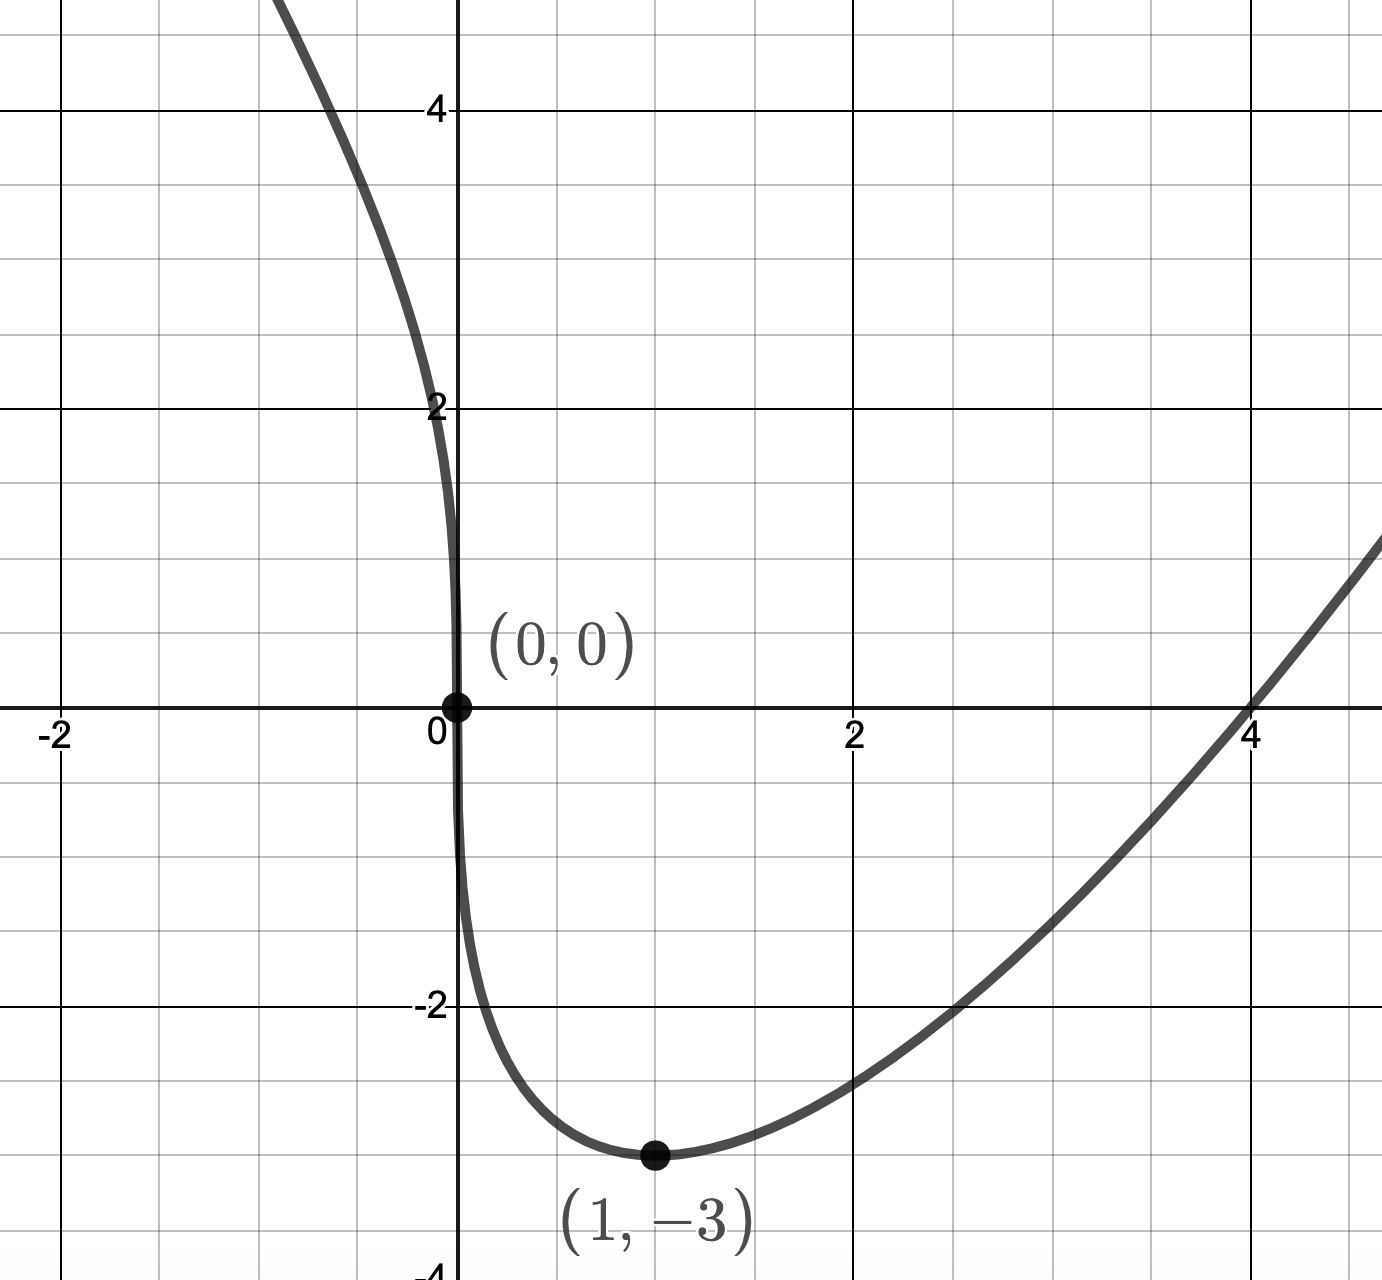
\includegraphics[width=3in]{./AppDerivativesGraphics/IncDecRoot.png}}

\end{enumerate}

\hfill \qed

\end{example}


\subsection{Concavity and the Second Derivative}
\label{concavity}

In section Section \ref{PowerFunctions}, we introduced the notion of \index{concavity}\textbf{concavity}.  In that section, we described curves as  being  \index{concave up}\index{concavity ! concave up}\textbf{concave up} over an interval if it resembles a  portion of a `$\smile$' shape and   \index{concave down}\index{concavity ! concave down}\textbf{concave down} over an interval if resembles part of a `$\frown$' shape. Now that we've had some exposure to Calculus, we can more precisely define these notions.

\medskip


%% \colorbox{ResultColor}{\bbm

\begin{definition}  \label{concavitydefn} Let $f$ be a differentiable function on an open interval  $I$.  Then $f$ is said to be:

\begin{itemize}

\item  \textbf{concave up} on $I$ if the tangent lines lie \textbf{below} the graph on $I$.

\item  \textbf{concave down} on $I$ if the tangent lines lie \textbf{above} the graph on $I$.

\smallskip

\end{itemize}

\end{definition}

%% \ebm}

\pagebreak

If we take the time to study a generic concave up curve, the `$\smile$' shape can be divided into a decreasing and increasing arc:

\begin{center}

\begin{multicols}{2}

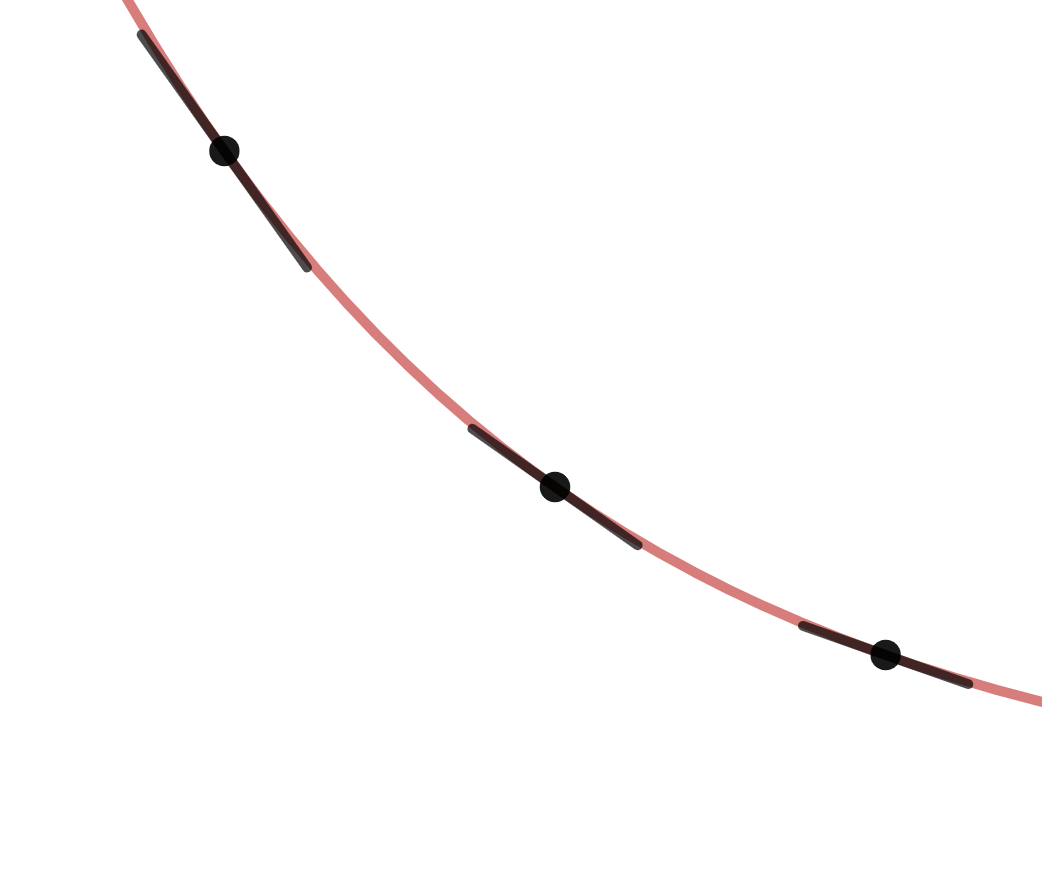
\includegraphics[width=1.5in]{./AppDerivativesGraphics/DecCU.png} 

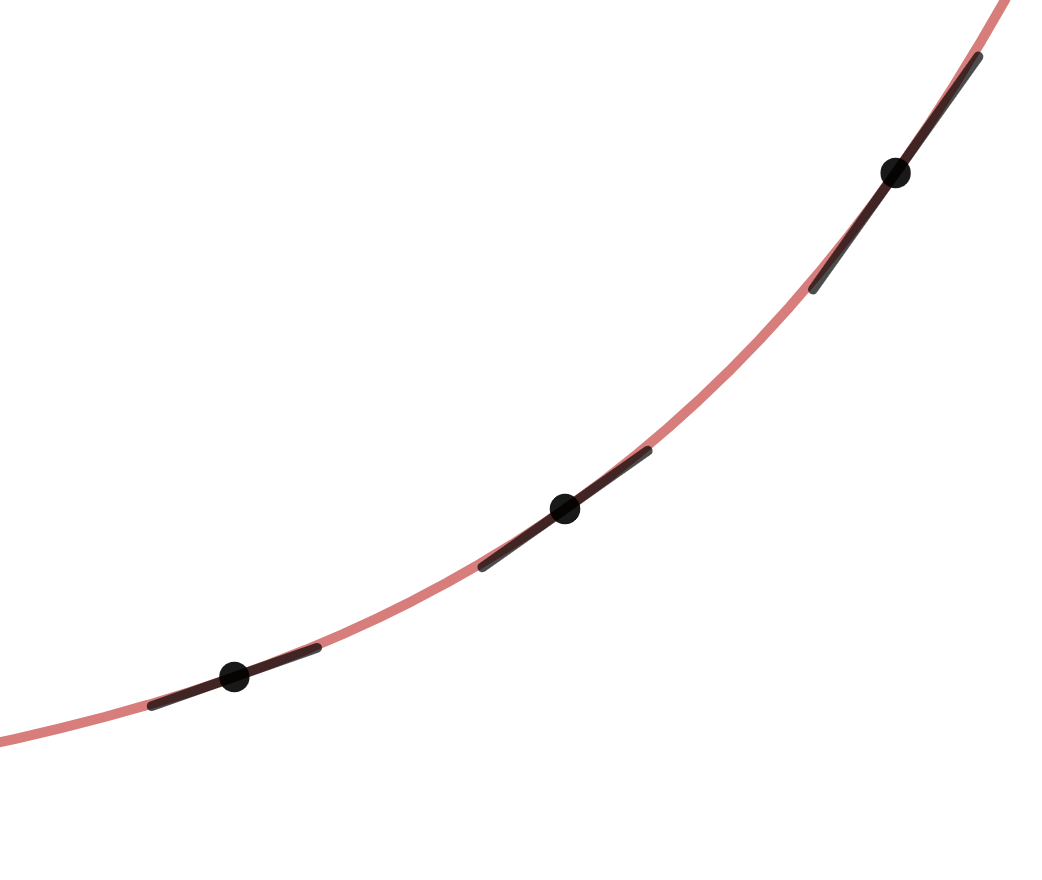
\includegraphics[width=1.5in]{./AppDerivativesGraphics/IncCU.png} 


\end{multicols}

\end{center}

\begin{center}

\begin{multicols}{2}

slopes are increasing towards $0$

slopes are increasing away from $0$

\end{multicols}

\end{center}

In both of these cases, the \textbf{slopes} of the tangent line are \textbf{increasing}.  

\medskip

Likewise, we can dissect a generic `$\frown$' shape curve into an increasing and decreasing arc:

\begin{center}

\begin{multicols}{2}

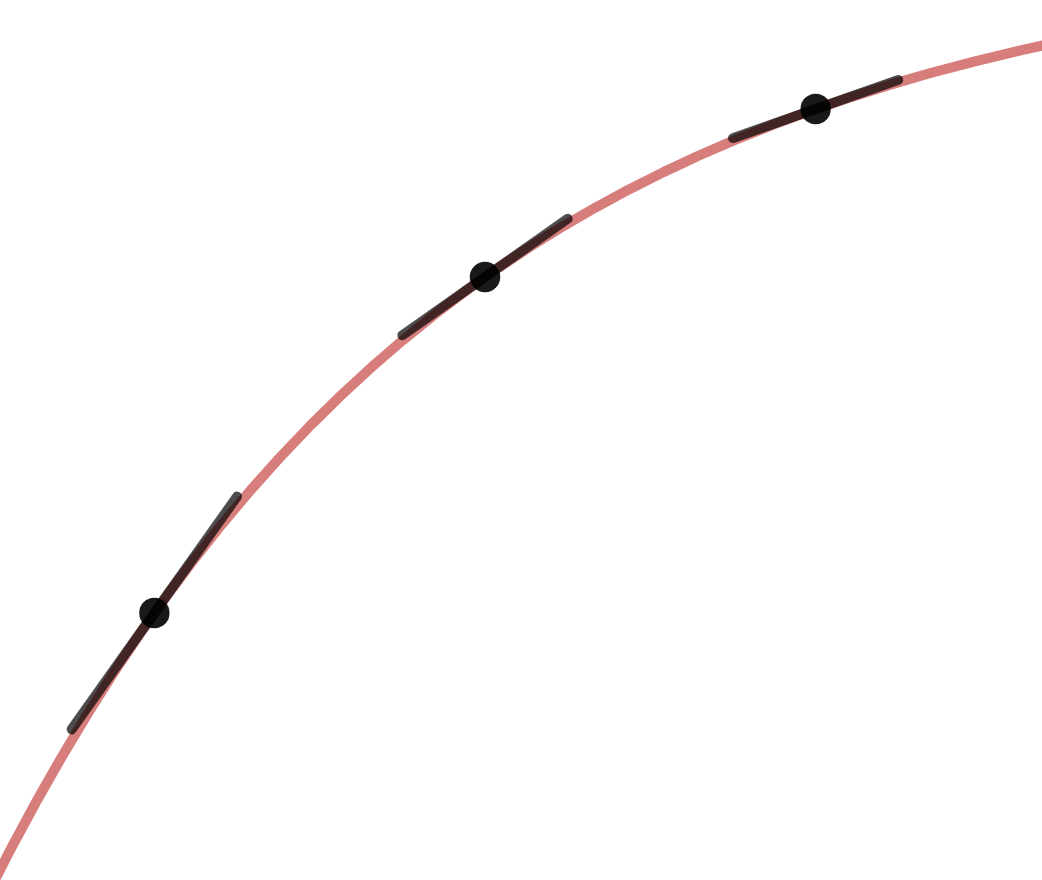
\includegraphics[width=1.5in]{./AppDerivativesGraphics/IncCD.png} 

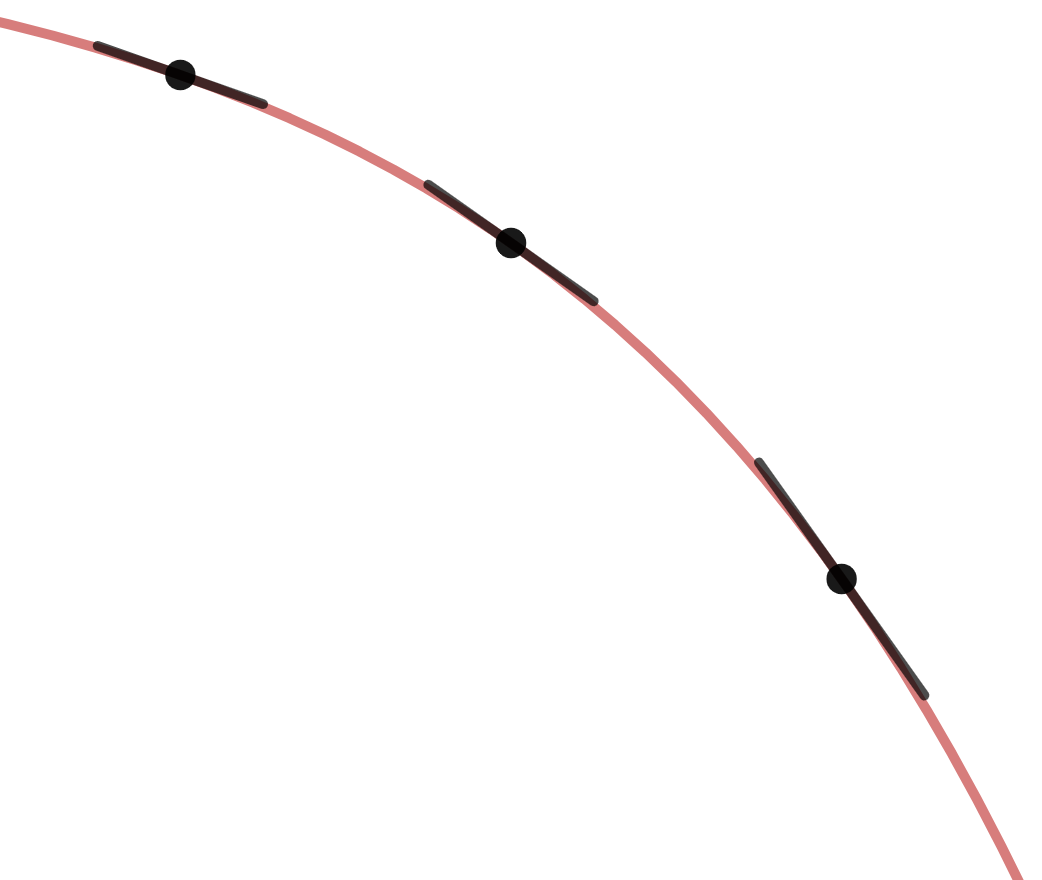
\includegraphics[width=1.5in]{./AppDerivativesGraphics/DecCD.png} 

\end{multicols}

\end{center}

\begin{center}

\begin{multicols}{2}

slopes are decreasing towards $0$

slopes are decreasing away from $0$

\end{multicols}

\end{center}

Here, the \textbf{slopes} of the tangent line are \textbf{decreasing}.  

\medskip

We know from Theorem \ref{firstderivatveandgraphs} that the derivative of a function can tell us where that function is increasing and decreasing.  Since the function which gives us the slopes of tangent lines is the derivative, $f'(x)$, we could use the derivative of $f'(x)$ to determine where the slopes of the tangent lines were increasing and decreasing.  This leads us to define the \index{second derivative}\index{derivative ! second}\textbf{second derivative}, $f''(x)$  as the derivative of $f'(x)$.

\medskip

We present the following theorem without proof, but hopefully sufficiently motivated. 

\medskip

%% \colorbox{ResultColor}{\bbm

\begin{theorem}  \label{secondderivatveandgraphs}   Suppose $f$ is twice differentiable on an open interval $I$:

\begin{itemize}

\item If $f''(x) > 0$ for all $x$ in $I$, then \textbf{slopes} are \textbf{increasing} and  $f$ is \textbf{concave up} on $I$.  

\item If $f''(x) < 0$ for all $x$ in $I$, then \textbf{slopes} are \textbf{decreasing} and  $f$ is \textbf{concave down} on $I$. 

\end{itemize}

\end{theorem}

%% \ebm}


\pagebreak

\begin{example}\label{polyconcavity} Let $f(x) = x^3 - 3x^2 - 9x+5$.  Use the fact that $f''(x) = 6x-6$ to find the intervals over which the graph of $f$ is concave up and concave down.

\medskip

{\bf Solution.}  To analyze the concavity of the graph of $f$, we need to make a sign diagram for $f''(x)$.  

\medskip

Solving $f''(x) = 6x-6 = 0$ gives $x=1$. We find $f''(0) =  6(0)-6 = (-)$ and $f''(2) = 6(2) - 6=  (+)$.  

\medskip

We have our sign diagram below on the left and our interpretation below on the right.

\begin{center}

\begin{multicols}{2}

\begin{mfpic}[15]{-6}{6}{-2}{2}
\arrow \reverse \arrow \polyline{(-5,0),(5,0)}
\xmarks{0}
\arrow \polyline{(-2,-1.5),(-2,-0.5)}
\arrow \polyline{(2,-1.5),(2,-0.5)}
\tlpointsep{4pt}
\axislabels {x}{{$1$} 0}
\tlabel[cc](-2,1){$(-)$}
\tlabel[cc](0,1){$0$}
\tlabel[cc](2,1){$(+)$}
\tlabel[cc](-2,-2.25){$0$}
\tlabel[cc](2,-2.25){$2$}
\tlabel[cc](6,1){$f''(x)$}
\tlabel[cc](6,-1){$x$}
%\tlabel[cc](6,0){$\infty$}
%\tlabel[cc](-6,0){$-\infty$}
\end{mfpic}

\begin{mfpic}[15]{-6}{6}{-2}{2}
\arrow \reverse \arrow \polyline{(-5,0),(5,0)}
\xmarks{0}
%\arrow \polyline{(-2,-1.5),(-2,-0.5)}
%\arrow \polyline{(2,-1.5),(2,-0.5)}
\tlpointsep{4pt}
\axislabels {x}{{$1$} 0}
\tlabel[cc](-2,1){\huge $\frown$}
%\tlabel[cc](0,1){$0$}
\tlabel[cc](2,1){\huge $\smile$}
%\tlabel[cc](-2,-2.25){$0$}
%\tlabel[cc](2,-2.25){$2$}
\tlabel[cc](6,1){$f(x)$}
\tlabel[cc](6,-1){$x$}
%\tlabel[cc](6,0){$\infty$}
%\tlabel[cc](-6,0){$-\infty$}
\end{mfpic}


\end{multicols}
\end{center}

We find $f$ is concave down on $(-\infty, 1)$ and concave up on $(1, \infty)$.  

\medskip

At $x=1$, the concavity changes.  We find $f(1) = (1)^3 - 3(1)^2 - 9(1)+5 = -6$ and we call the point $(1, -6)$ an \textbf{inflection point}.  In this case since the concavity changes from concave down to concave up, the point $(1,-6)$ is the point on the graph of $y=f(x)$ were the slopes stop decreasing and start to increase.

\medskip

A quick check using desmos confirms our results.

\medskip

\centerline{ 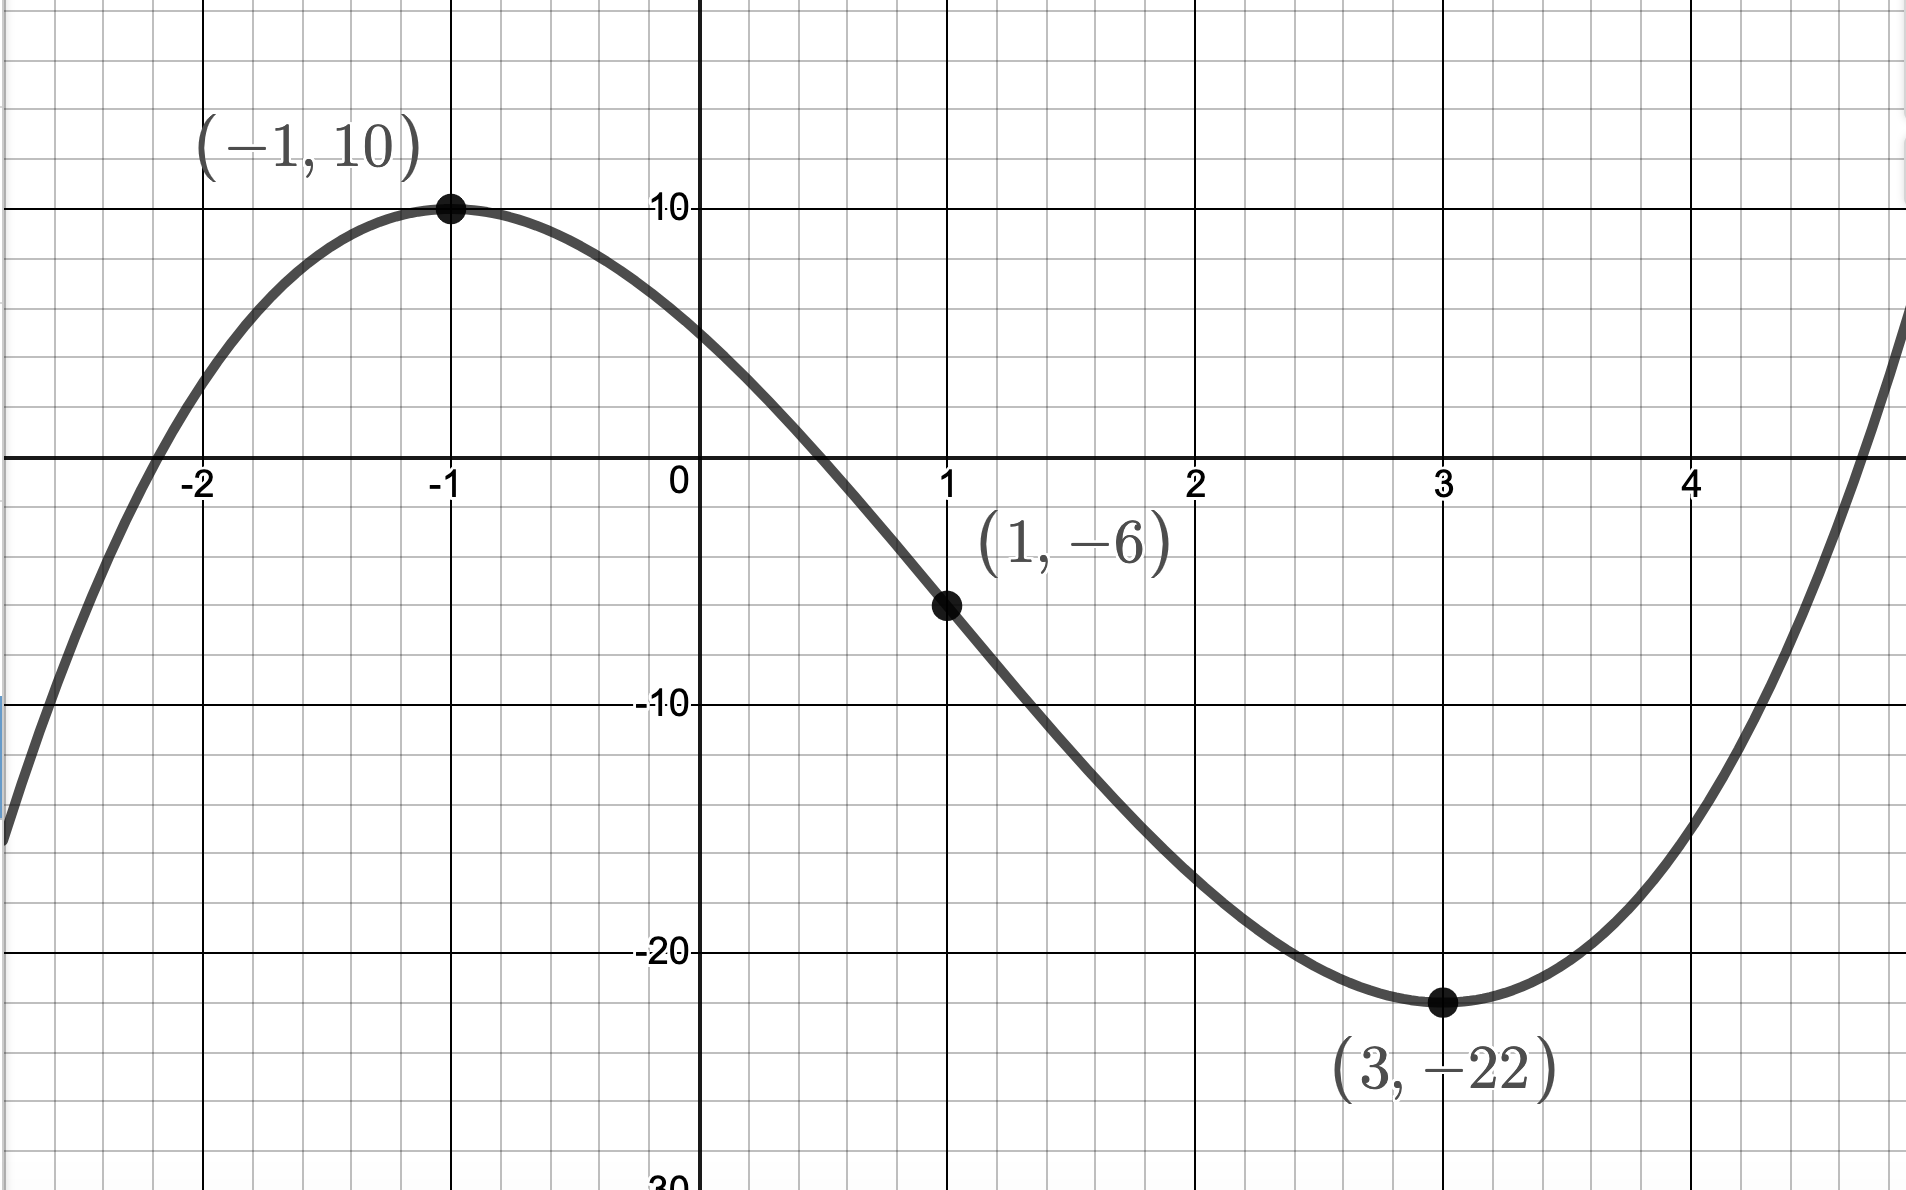
\includegraphics[width=4in]{./AppDerivativesGraphics/ConcavityPoly.png}}

\hfill \qed

\end{example}

\medskip

Note that we can use concavity to help us distinguish local extrema.  

\medskip

For the function above, both $f'(-1) = 0$ and $f'(3) = 0$.  Note that $f''(-1) < 0$ which means $f$ is concave down there. This forces $f$ to have a local maximum at $(-1,6)$.  Likewise, $f''(3) > 0$ which means $f$ is concave up there.  This forces $f$ to have a local minimum at $(3,-22)$.  We generalize this observation below.

\medskip



%% \colorbox{ResultColor}{\bbm

\begin{theorem}  \label{secondderivatvetest}   \textbf{The Second\footnote{Now you know why we titled Theorem \ref{firstderivatvetest} the `First' Derivative Test for Local Extrema.} Derivative Test for Local Extrema:}  Suppose $f$ is differentiable on an open interval $I$ containing $c$ and $f'(c) = 0$:

\begin{itemize}

\item If $f''(c) > 0$ then $f$ has a local minimum at $x=c$.

\item If $f''(c) < 0$ then $f$ has a local maximum at $x=c$.

\item If $f''(c) = 0$ then the test is inconclusive.  $f$ may or may not have a local extremum at $x=c$.  

(In this case, we would appeal to the first derivative test.)

\end{itemize}
\end{theorem}

%% \ebm}



\medskip

\begin{example} \label{powerfcnconcavity}  Let $f(x) = x^{4/3} - 4x^{1/3}$.   Use the fact that $f''(x) =  \frac{4}{9} x^{-2/3} + \frac{8}{9} x^{-5/3}$ to help you find:

\begin{enumerate}

\item  the open intervals over which the graph of $f$ is concave up and concave down.

\item  the inflection points in the graph.

\end{enumerate}

\medskip

{\bf Solution.}

\begin{enumerate} \item  As in Example \ref{powerfcnincdec}, our first step is to  rewrite  $f''(x) =  \frac{4}{9} x^{-2/3} + \frac{8}{9} x^{-5/3}$  as a single fraction:


\[ f''(x) = \dfrac{4}{9} x^{-2/3} + \dfrac{8}{9} x^{-5/3} = \dfrac{4}{9x^{2/3}} + \dfrac{8}{9x^{5/3}} =  \dfrac{4}{9x^{2/3}} \cdot \dfrac{x^{3/3}}{x^{3/3}}+ \dfrac{8}{9x^{5/3}}  =  \dfrac{4x}{9x^{5/3}} + \dfrac{8}{9x^{5/3}}   =  \dfrac{4x+8}{9x^{5/3}}  \]

\medskip

We see $f''(x) =  \frac{4x+8}{9x^{5/3}} $ is undefined when $9x^{5/3}= 0$, that is, when $x = 0$.  

\medskip

Solving $f''(x) =  \frac{4x+8}{9x^{5/3}}  = 0$ gives $4x+8 = 0$ so $x = -2$. 

\newpage

Going through the usual routine, we obtain our sign diagram for $f''(x)$ is below.

\medskip

\begin{center}

\begin{multicols}{2}

\begin{mfpic}[15]{-6}{6}{-2}{2}
\arrow \reverse \arrow \polyline{(-5,0),(5,0)}
\xmarks{-2,2}
\arrow \polyline{(-3.5,-1.5),(-3.5,-0.5)}
\arrow \polyline{(0,-1.5),(0,-0.5)}
\arrow \polyline{(3.5,-1.5),(3.5,-0.5)}
\tlpointsep{4pt}
\axislabels {x}{{$-2 \hspace{7 pt}$} -2, {$0$} 2}
\tlabel[cc](-3.5,1){$(+)$}
\tlabel[cc](-2,1){$0$}
\tlabel[cc](0,1){$(-)$}
\tlabel[cc](2,1){\textinterrobang}
\tlabel[cc](3.5,1){$(+)$}
\tlabel[cc](-3.75,-2.25){$-1$}
\tlabel[cc](0,-2.25){$\frac{1}{2}$}
\tlabel[cc](3.6,-2.25){$2$}
\tlabel[cc](6,1){$f''(x)$}
\tlabel[cc](6,-1){$x$}
%\tlabel[cc](6,0){$\infty$}
%\tlabel[cc](-6,0){$-\infty$}
\end{mfpic}

\begin{mfpic}[15]{-6}{6}{-2}{2}
\arrow \reverse \arrow \polyline{(-5,0),(5,0)}
\xmarks{-2,2}
%\arrow \polyline{(-3.5,-1.5),(-3.5,-0.5)}
%\arrow \polyline{(0,-1.5),(0,-0.5)}
%\arrow \polyline{(3.5,-1.5),(3.5,-0.5)}
\tlpointsep{4pt}
\axislabels {x}{{$-2 \hspace{7 pt}$} -2, {$0$} 2}
\tlabel[cc](-3.5,1){\Huge $\smile$}
%\tlabel[cc](-2,1){?}
\tlabel[cc](0,1){\Huge $\frown$}
%\tlabel[cc](2,1){?}
\tlabel[cc](3.5,1){\Huge $\smile$}
%\tlabel[cc](-3.75,-2.25){$-3$}
%\tlabel[cc](0,-2.25){$0$}
%\tlabel[cc](3.6,-2.25){$4$}
\tlabel[cc](6,1){$f(x)$}
\tlabel[cc](6,-1){$x$}
%\tlabel[cc](6,0){$\infty$}
%\tlabel[cc](-6,0){$-\infty$}
\end{mfpic}


\end{multicols}
\end{center}

We see $f$ is concave up on $(-\infty, -2)$ and again from $(0, \infty)$.  $f$ is concave down on $(-2,0)$.

\item  Since $f$ changes concavity at both $x=-2$ and $x=0$, we have inflection point at both of these values.  

\medskip

We find:  $f(-2) = (-2)^{4/3} - 4(-2)^{1/3} = 2 (2)^{1/3} + 4 (2)^{1/3} = 6 (2)^{1/3}$. So $\left(-2, 6 (2)^{1/3} \right)$ is one inflection point.  When $x = 0$, $f(0) = (0)^{4/3} - 4(0)^{1/3}  = 0$, so $(0,0)$ is the other inflection point.  

\medskip
Checking with desmos, it's not apparent that the graph of $y=f(x)$ is concave up for $x<-2$.  We invite the reader to graph $f$ and zoom out to see that characteristic of the graph.


\medskip

\centerline{ 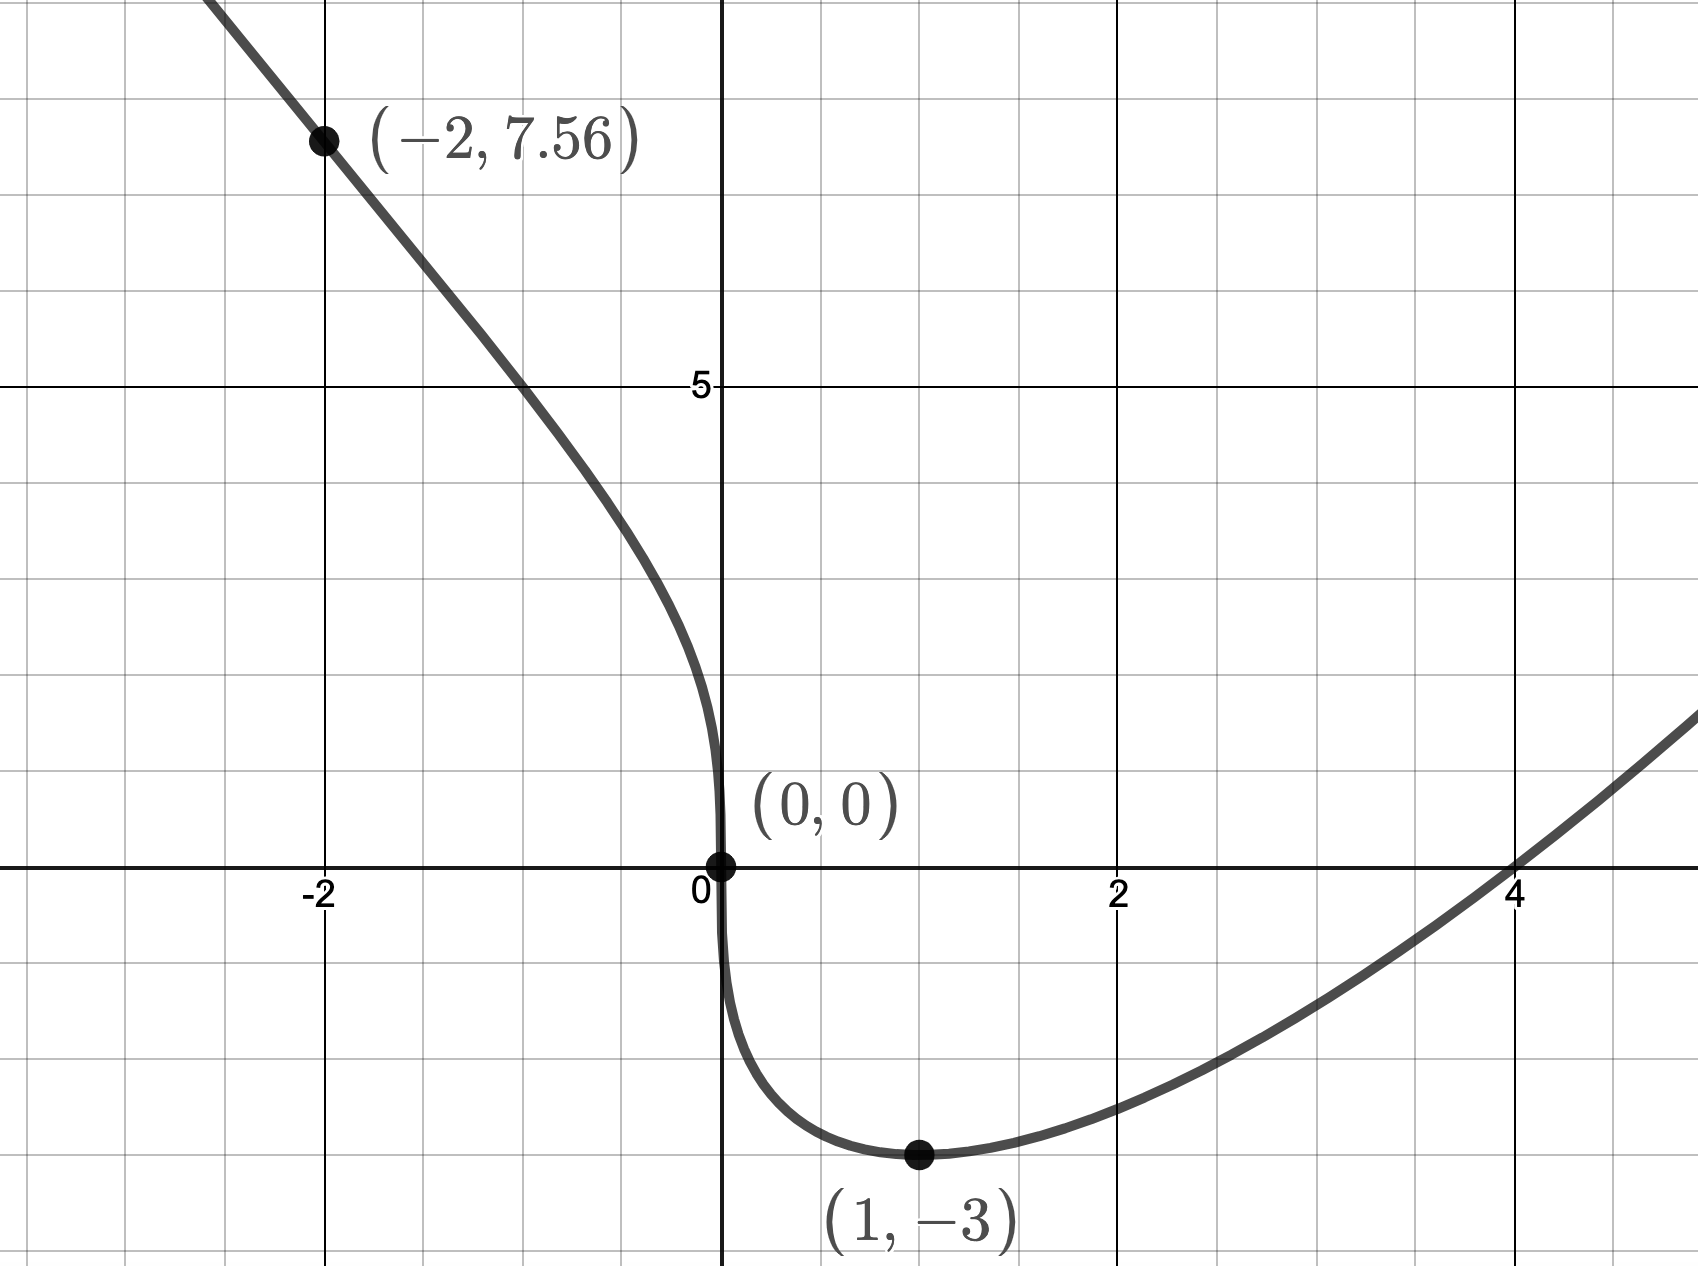
\includegraphics[width=3in]{./AppDerivativesGraphics/ConcavityRoot.png}}

\hfill \qed



\end{enumerate}

\end{example}

\medskip

Our last example offers a twist on these sorts of curve-sketching problems.

\pagebreak

\begin{example}\label{graphfromderivativegraphex} Below is the graph of the \textbf{derivative} of a function.  Assume as $x \rightarrow \pm \infty$, $f'(x) \rightarrow -\infty$.


\begin{center}

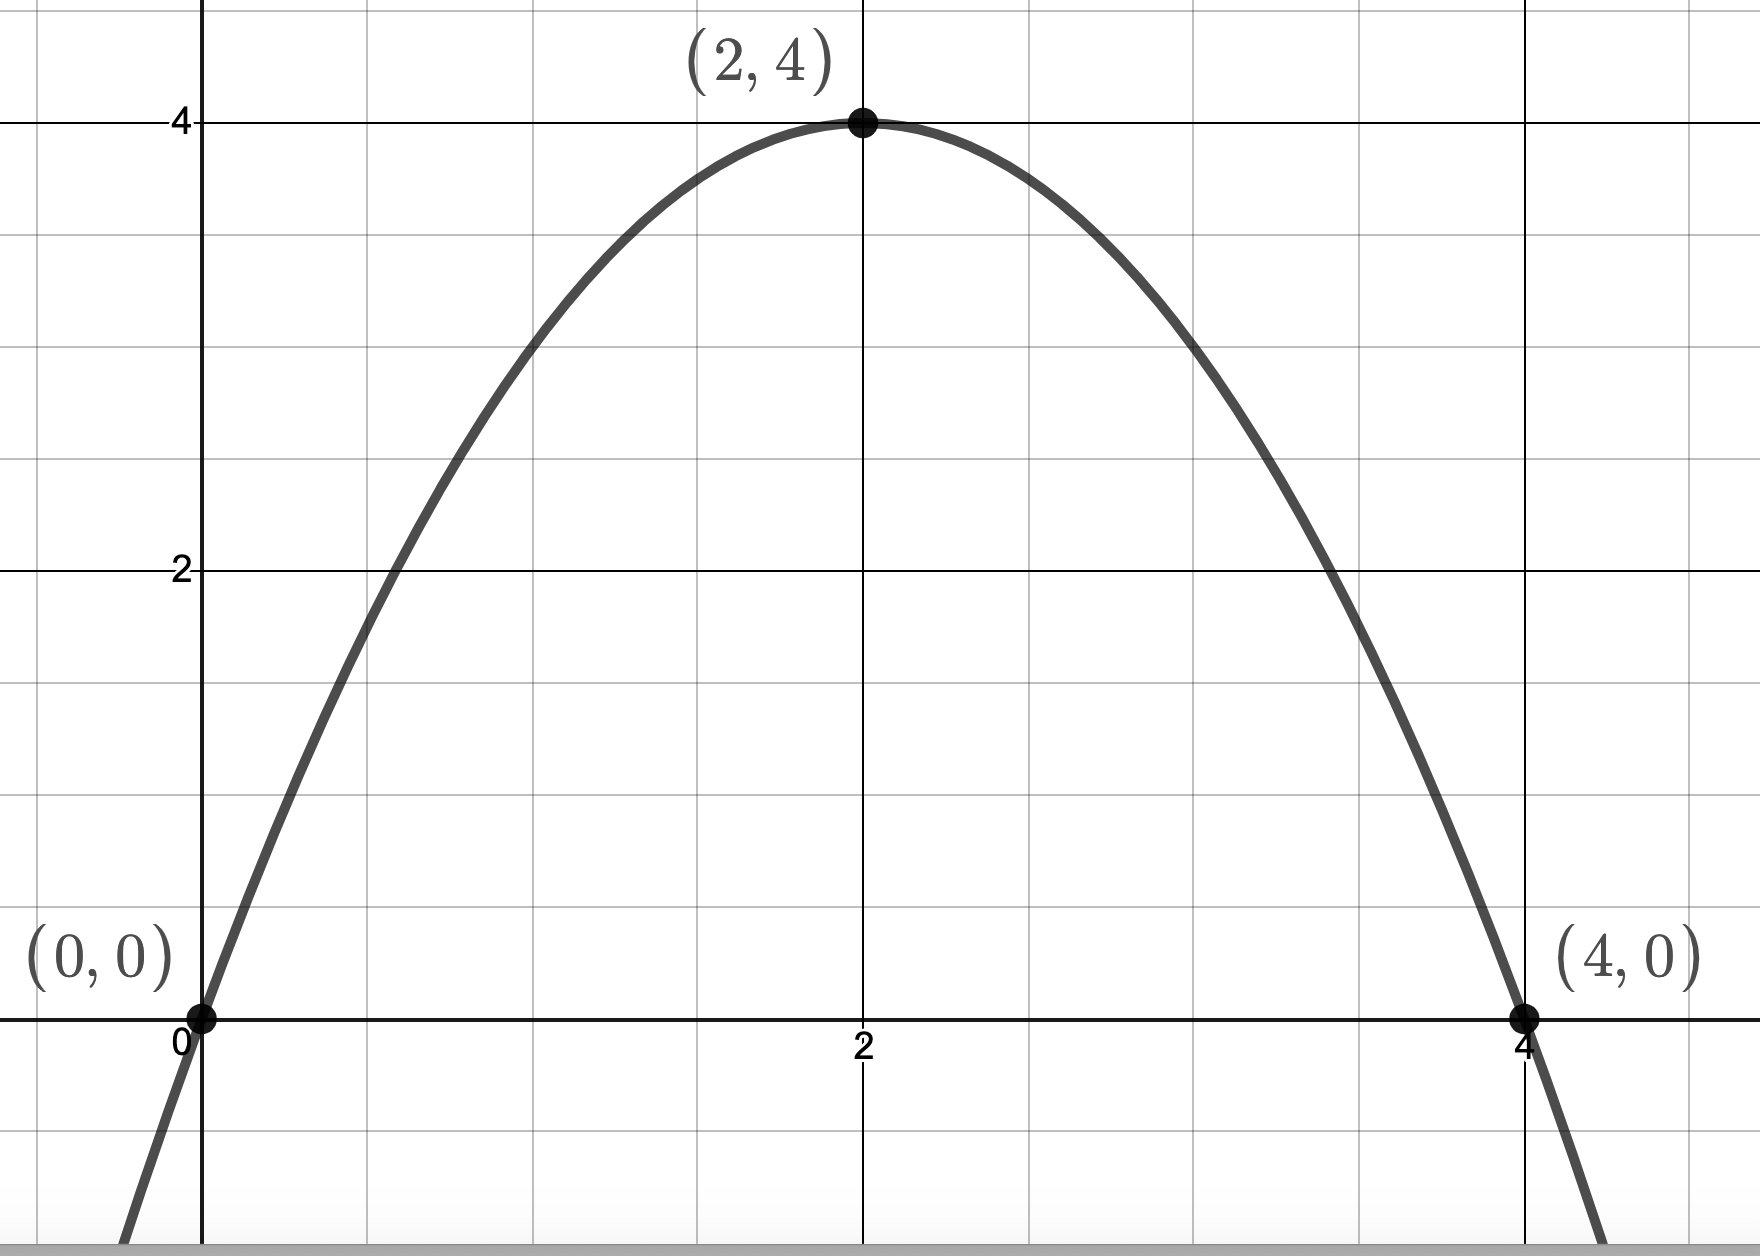
\includegraphics[width=4in]{./AppDerivativesGraphics/derivgraph.png}

The graph of $y=f'(x)$

\end{center}

\begin{enumerate}

\item  Use the graph of $y=f'(x)$ to determine the open intervals where $f$ is increasing and decreasing.  

\medskip

Find the $x$-coordinates of the local extrema.

\medskip

\item  Use the graph of $y=f'(x)$ make a sign diagram for $y=f''(x)$.

\medskip

\item  List the open intervals over which the graph of $f$ is concave up and concave down.  

\medskip

Find the $x$-coordinates of the inflection points. 

\medskip

\item  Sketch a possible graph of $y = f(x)$.

\end{enumerate}

\medskip

{\bf Solution.}

\begin{enumerate}

\item  Recall from algebra, the solutions to $f'(x) < 0$ are the $x$-values where the graph of $y = f'(x)$  is below the $x$-axis.  This happens on the intervals $(-\infty, 0)$ and $(4, \infty)$, so this means  $f$ is decreasing here.  

\medskip

Likewise,  the solutions to $f'(x) > 0$ are the $x$-values where $y=f'(x)$ is above the $x$-axis.  This happens on the interval $(0,4)$, so $f$ is increasing here.  


\medskip

Since $f$ goes from decreasing to the left of $x=0$ to increasing to the right of $x=0$, $f$ has a local minimum at $x=0$.  Since $f$ goes from increasing to the left of $x=4$ to decreasing to the right of $x=4$, $f$ has a local maximum at $x=4$.

\pagebreak


\item  Since $f''(x)$ is the derivative of $f'(x)$, we know $f''(x) > 0$ on $(-\infty, 2)$ since $f'(x)$ is increasing there.  We see $f''(2) = 0$ since $f'(x)$ is locally flat at $(2,4)$.  Lastly, we see $f''(x) < 0$ on $(2, \infty)$ since $f'(x)$ is decreasing there.  We put all this together in a sign diagram below.

\medskip

\begin{center}

\begin{multicols}{2}

\begin{mfpic}[15]{-6}{6}{-2}{2}
\arrow \reverse \arrow \polyline{(-5,0),(5,0)}
\xmarks{0}
%\arrow \polyline{(-2,-1.5),(-2,-0.5)}
%\arrow \polyline{(2,-1.5),(2,-0.5)}
\tlpointsep{4pt}
\axislabels {x}{{$2$} 0}
\tlabel[cc](-2,1){$(+)$}
\tlabel[cc](0,1){$0$}
\tlabel[cc](2,1){$(-)$}
%\tlabel[cc](-2,-2.25){$0$}
%\tlabel[cc](2,-2.25){$3$}
\tlabel[cc](6,1){$f''(x)$}
\tlabel[cc](6,-1){$x$}
%\tlabel[cc](6,0){$\infty$}
%\tlabel[cc](-6,0){$-\infty$}
\end{mfpic}

\begin{mfpic}[15]{-6}{6}{-2}{2}
\arrow \reverse \arrow \polyline{(-5,0),(5,0)}
\xmarks{0}
%\arrow \polyline{(-2,-1.5),(-2,-0.5)}
%\arrow \polyline{(2,-1.5),(2,-0.5)}
\tlpointsep{4pt}
\axislabels {x}{{$2$} 0}
\tlabel[cc](-2,1){\Huge $\smile$}
%\tlabel[cc](0,1){$\rightarrow$}
\tlabel[cc](2,1){\Huge $\frown$}
%\tlabel[cc](-2,-2.25){$0$}
%\tlabel[cc](2,-2.25){$2$}
\tlabel[cc](6,1){$f(x)$}
\tlabel[cc](6,-1){$x$}
%\tlabel[cc](6,0){$\infty$}
%\tlabel[cc](-6,0){$-\infty$}
\end{mfpic}


\end{multicols}

\end{center}


\item   We have $f$ is concave up on $(-\infty, 2)$ and concave down on $(2, \infty)$.

\medskip

Since $f$ changes concavity at $x=2$, there is an inflection point there.

\medskip

\item   A plausible graph of $y = f(x)$  is below.  We cannot determine any $y$-coordinates (why not?)


\begin{center}

 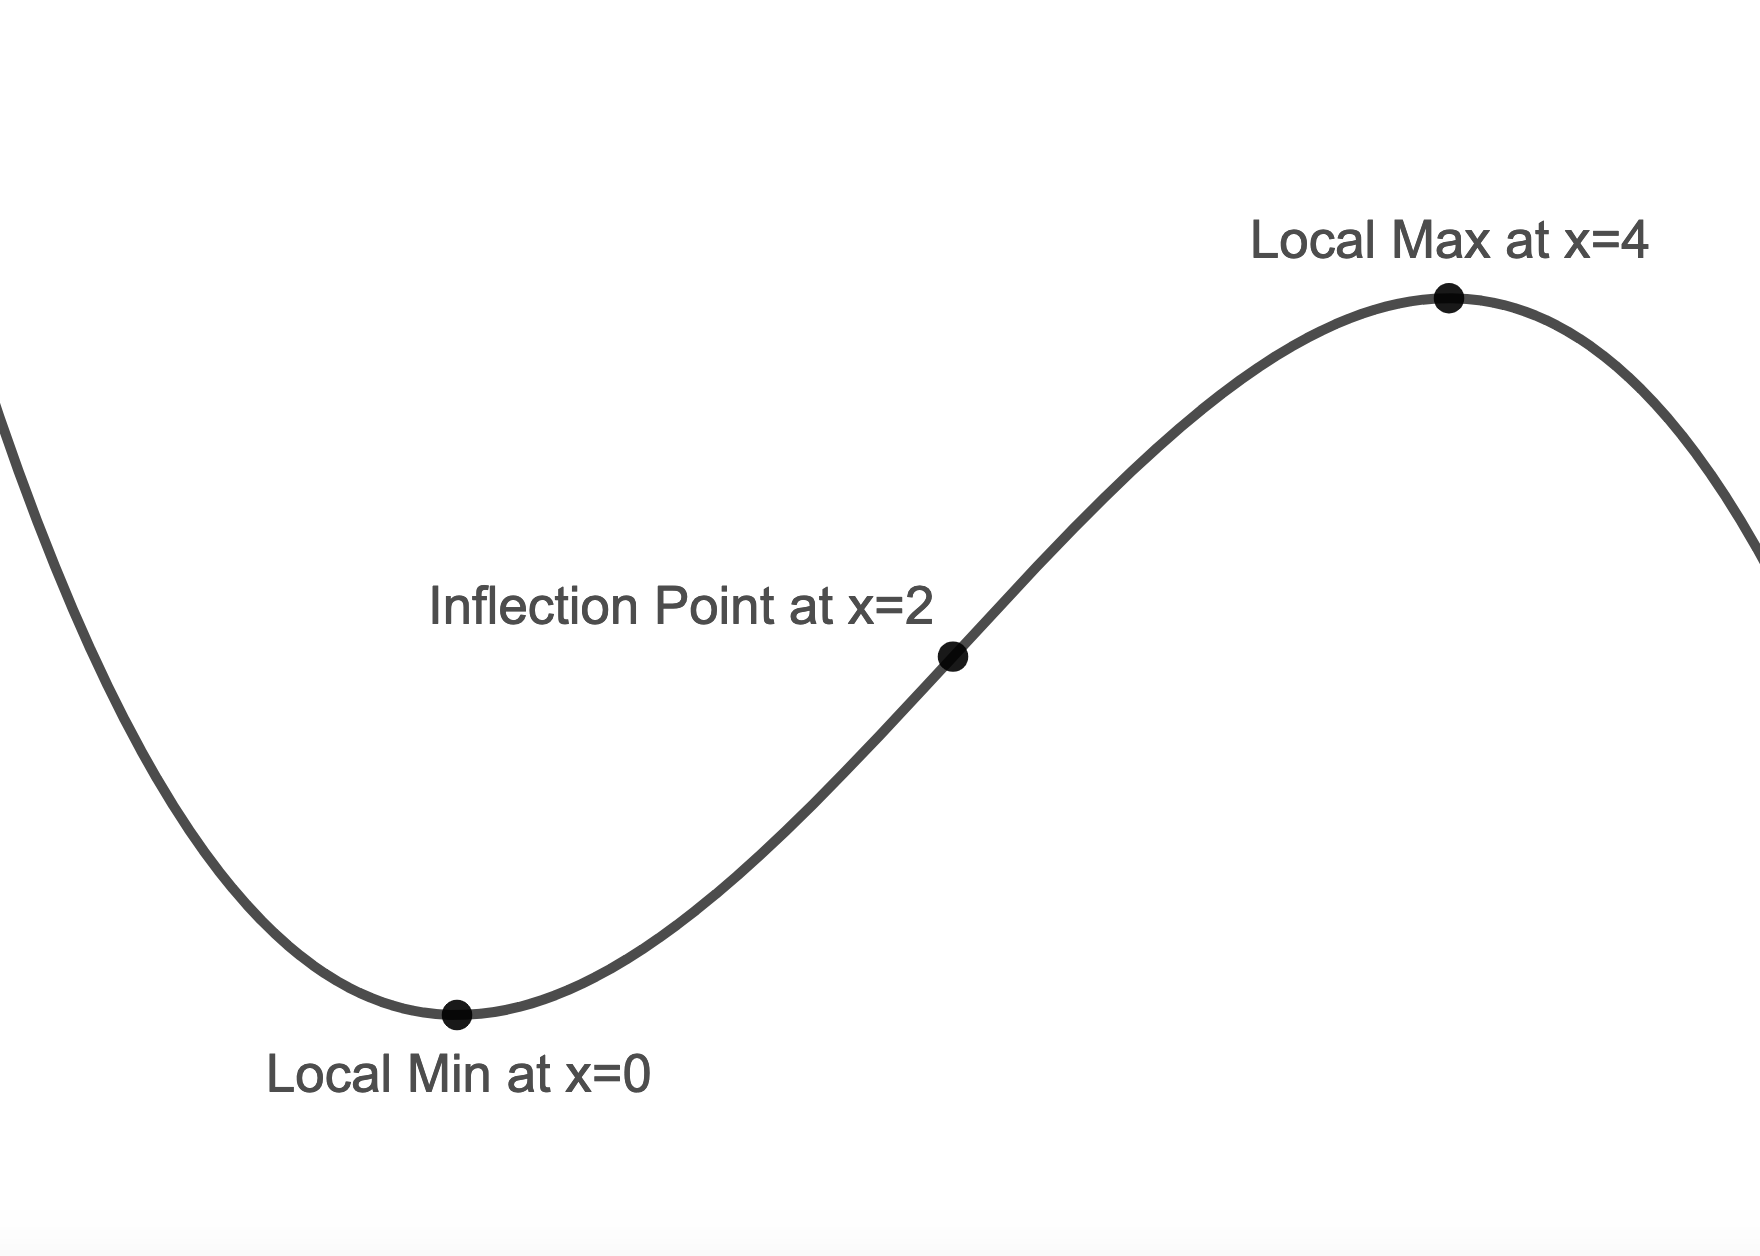
\includegraphics[width=4in]{./AppDerivativesGraphics/original.png}
 
 A possible graph of $y = f(x)$
 
 \end{center}


\end{enumerate}

\hfill \qed

\end{example}



%\subsection{Related Rates}
%\label{relatedrates}

%\subsection{Marginal Analysis}
%\label{marginals}




\newpage

\subsection{Exercises}
%% SKIPPED %% \label{ExercisesforAppDerivatives}

\begin{itemize}
\item basic curve sketching
\item revisit `unusual steepness' from Ch 4
\item  Vertex formula, revisited
\item  inflection point of cubic (pattern with vertex formula and zero of linear.)
\end{itemize}

\closegraphsfile

\end{document}
